% -*- latex -*-
%%%%%%%%%%%%%%%%%%%%%%%%%%%%%%%%%%%%%%%%%%%%%%%%%%%%%%%%%%%%%%%%
%%%%
%%%% This TeX file is part of the course
%%%% Introduction to Scientific Programming in C++/Fortran2003
%%%% copyright 2017-9 Victor Eijkhout eijkhout@tacc.utexas.edu
%%%%
%%%% arrayf.tex : arrays in Fortran
%%%%
%%%%%%%%%%%%%%%%%%%%%%%%%%%%%%%%%%%%%%%%%%%%%%%%%%%%%%%%%%%%%%%%

Array handling in Fortran is similar to C++ in some ways, but there
are differences, such as that  Fortran indexing starts at~1, rather
than~0. More importantly, Fortran has better handling of
multi-dimensional arrays, and it is easier to manipulate whole arrays.

\Level 0 {Static arrays}

The preferred way for specifying an array size is:

\begin{block}{Fortran dimension}
  \label{sl:farray-dimension}
Preferred way of creating arrays through \indextermfort{dimension}
keyword:
\begin{lstlisting}
real(8), dimension(100) :: x,y
\end{lstlisting}
One-dimensional arrays of size~100.

Older mechanism works too:
\begin{lstlisting}
integer :: i(10,20)
\end{lstlisting}
Two-dimensional array of size~$10\times 20$.

These arrays are statically defined, and only live inside their
program unit.
\end{block}

Such an array, with size explicitly indicated, is called a
\indextermsub{static}{array} or \indextermsub{automatic}{array}.
(See section~\ref{sec:allocatable} for
dynamic arrays.)

\begin{block}{1-based Indexing}
  \label{sl:farray-base1}
Array indexing in Fortran is 1-based by default:
\begin{lstlisting}
integer,parameter :: N=8
real(4),dimension(N) :: x
do i=1,N
  ... x(i) ...
\end{lstlisting}
Note the use of \lstinline{parameter}:
\indexterm{compile-time constant}
\end{block}

\begin{block}{Lower bound}
  \label{sl:farray-lower}
Unlike C++, Fortran can specify the lower bound explicitly:
\begin{lstlisting}
real,dimension(-1:7) :: x
do i=-1,7
  ... x(i) ...
\end{lstlisting}
Safer:
\snippetwithoutput{lubound}{arrayf}{lubound}
\end{block}

Such arrays, as in~C++, obey the scope: they disappear at the end of
the program or subprogram.

\Level 1 {Initialization}

There are various syntaxes for \indextermbus{array}{initialization},
including the use of
\emph{implicit do-loops}\index{do loop!implicit!and array initialization}:
%
\begin{block}{Array initialization}
  \label{sl:farray-init}
  \verbatimsnippet{farrayinit}
\end{block}

\Level 1 {Array sections}

Fortran is more sophisticated than C++ in how it can handle arrays as
a whole. For starters, you can assign one array to another:

\begin{lstlisting}
real*8, dimension(10) :: x,y
x = y
\end{lstlisting}

This obviously requires the arrays to have the same size.
You can assign subarrays, or \emph{array sections}\index{index!section},
as long as they have the same shape. This uses a colon syntax.

\begin{slide}{Array sections example}
  \label{sl:farray-section}
  Use the colon notation to indicate ranges:
\begin{lstlisting}
real(4),dimension(4) :: y
real(4),dimension(5) :: x
x(1:4) = y
x(2:5) = x(1:4)
\end{lstlisting}
\end{slide}

\begin{block}{Array sections}
  \label{sl:farray-sections}
  \begin{itemize}
  \item {\tt :} %\n{:}
    to get all indices,
  \item {\tt :n} % \n{:n}
    to get indices up to~\n{n},
  \item {\tt n:} % \n{n:}
    to get indices \n{n} and up.
  \item {\tt m:n}
    indices in range \n{m,...,n}.
  \end{itemize}
\end{block}

\begin{block}{Use of sections}
  \label{sl:farray-sectionassign}
  \snippetwithoutput{fsectionassign}{arrayf}{sectionassign}
\end{block}

\begin{exercise}
  \label{ex:sect-vs-loop}
  Code out the above array assignment with an explicit,
  indexed loop. Do you get the same output? Why? What conclusion do
  you draw about internal mechanisms used in array sections?
\end{exercise}

You can even use a stride:

\begin{block}{Strided sections}
  \label{sl:farray-strideassign}
  \snippetwithoutput{fsectionmg}{arrayf}{sectionmg}
\end{block}

\begin{exercise}
  \label{ex:farray-shift}

  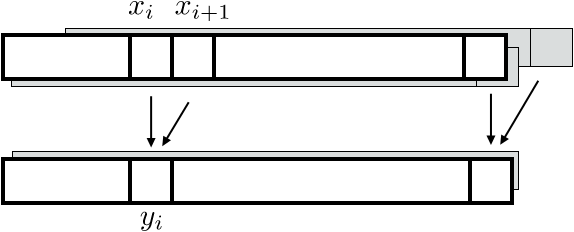
\includegraphics[scale=.3]{yx_average}

  Code $\forall_i\colon y_i=(x_i+x_{i+1})/2$:
  \begin{itemize}
  \item First with a do loop; then
  \item in a single array assignment statement by using sections.
  \end{itemize}
  Initialize the array \n{x} with values that allow you to check the
  correctness of your code.
\end{exercise}

\Level 1 {Integer arrays as indices}

\begin{block}{Index arrays}
  \label{sl:farray-indexarray}
\begin{lstlisting}
integer,dimension(4) :: i = [2,4,6,8]
real(4),dimension(10) :: x
print *,x(i)
\end{lstlisting}
\end{block}

\Level 0 {Multi-dimensional}

Arrays above had `\emph{rank}\index{array!rank}~one'. The rank is
defined as the number of indices you need to address the
elements. Calling this the `dimension' of the array can be confusing, but
we will talk about the first and second dimension of the array.

A rank-two array, or matrix, is defined like this:
\begin{block}{Multi-dimension arrays}
  \label{sl:farray-2d}
\begin{lstlisting}
real(8),dimension(20,30) :: array
array(i,j) = 5./2
\end{lstlisting}
\end{block}

With multidimensional arrays we have to worry how they are stored in
memory. Are they stored row-by-row, or column-by-column? In Fortran
the latter choice, also known as \indextermdef{column-major} storage,
is used; see figure~\ref{fig:column-major}.

\begin{figure}[ht]
  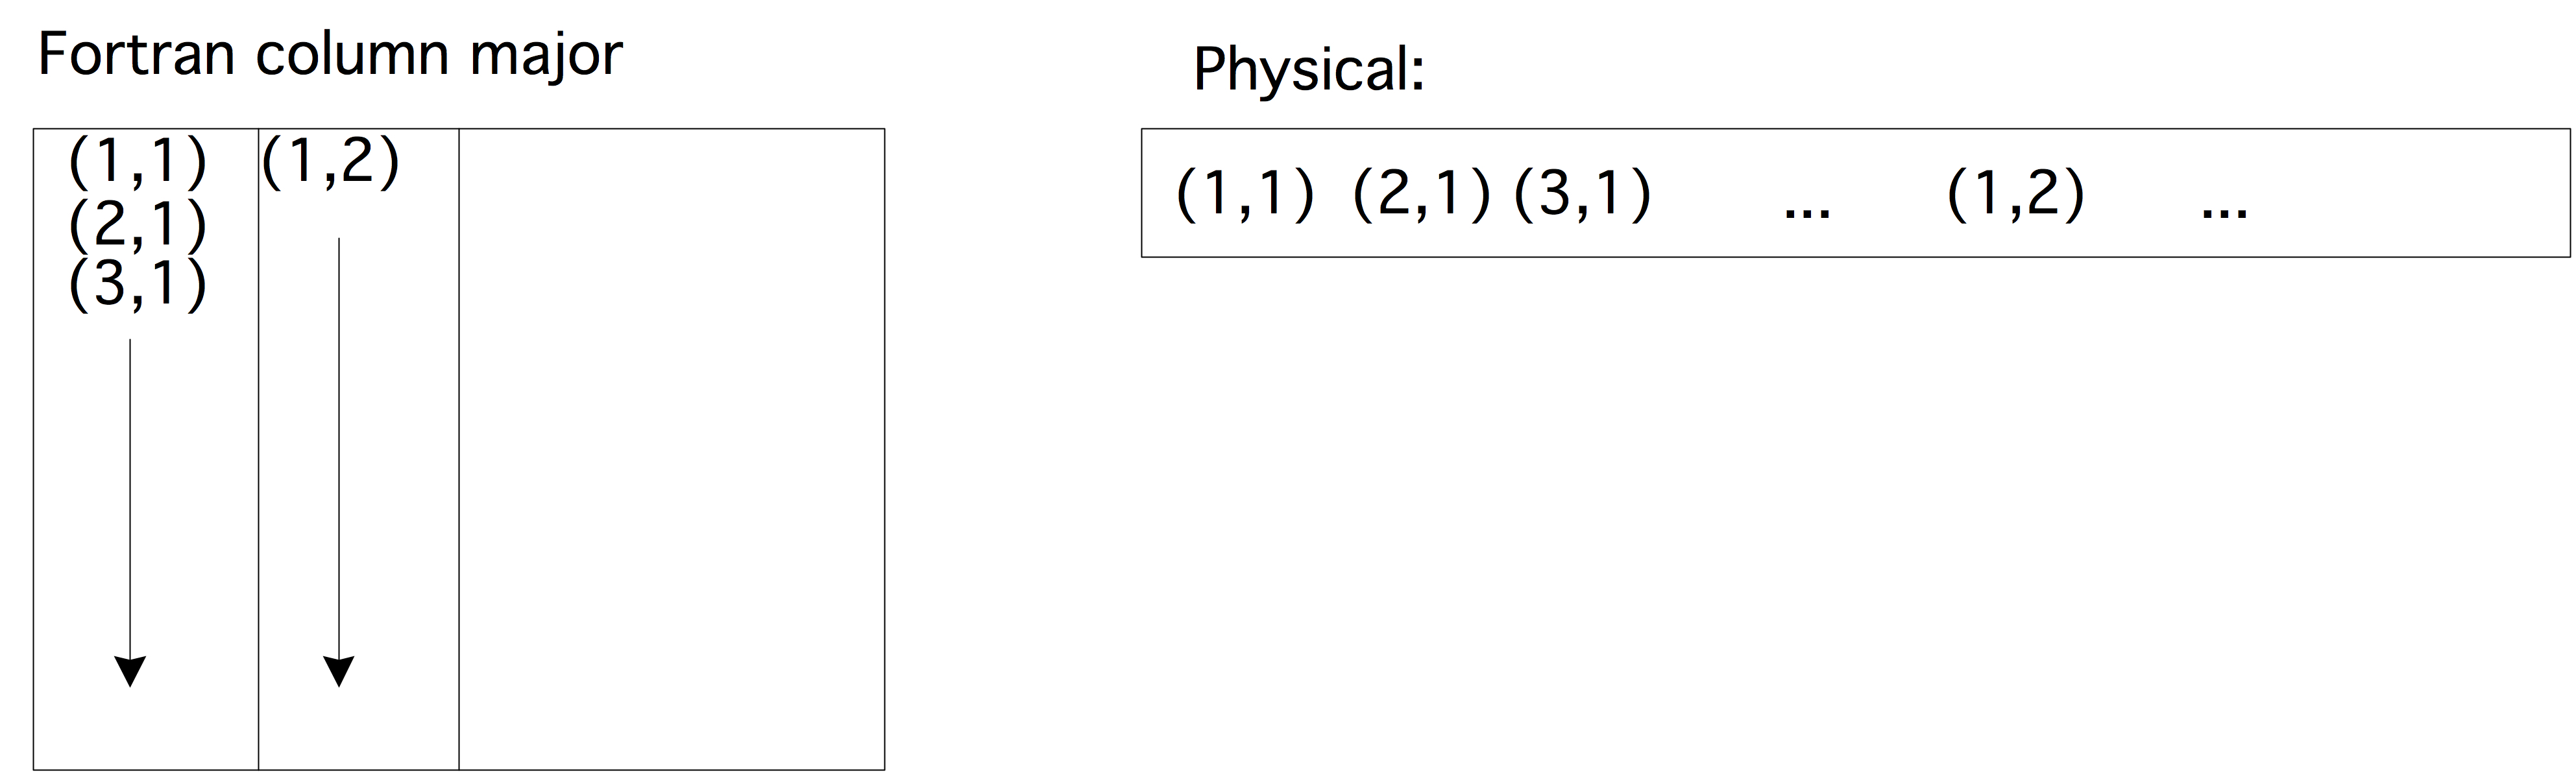
\includegraphics[scale=.1]{arraybycol}
  \caption{Column-major storage in Fortran}
  \label{fig:column-major}
\end{figure}

To traverse the elements as they are stored in memory, you would need
the following code:
\begin{lstlisting}
do col=1,size(A,2)
  do row=1,size(A,1)
    .... A(row,col) .....
  end do
end do
\end{lstlisting}
This is sometimes described as `First index varies quickest'.

\begin{slide}{Array layout}
  \label{sl:farray-layout}
  Sometimes you have to take into account how a higher rank array
  is laid out in (linear) memory:

  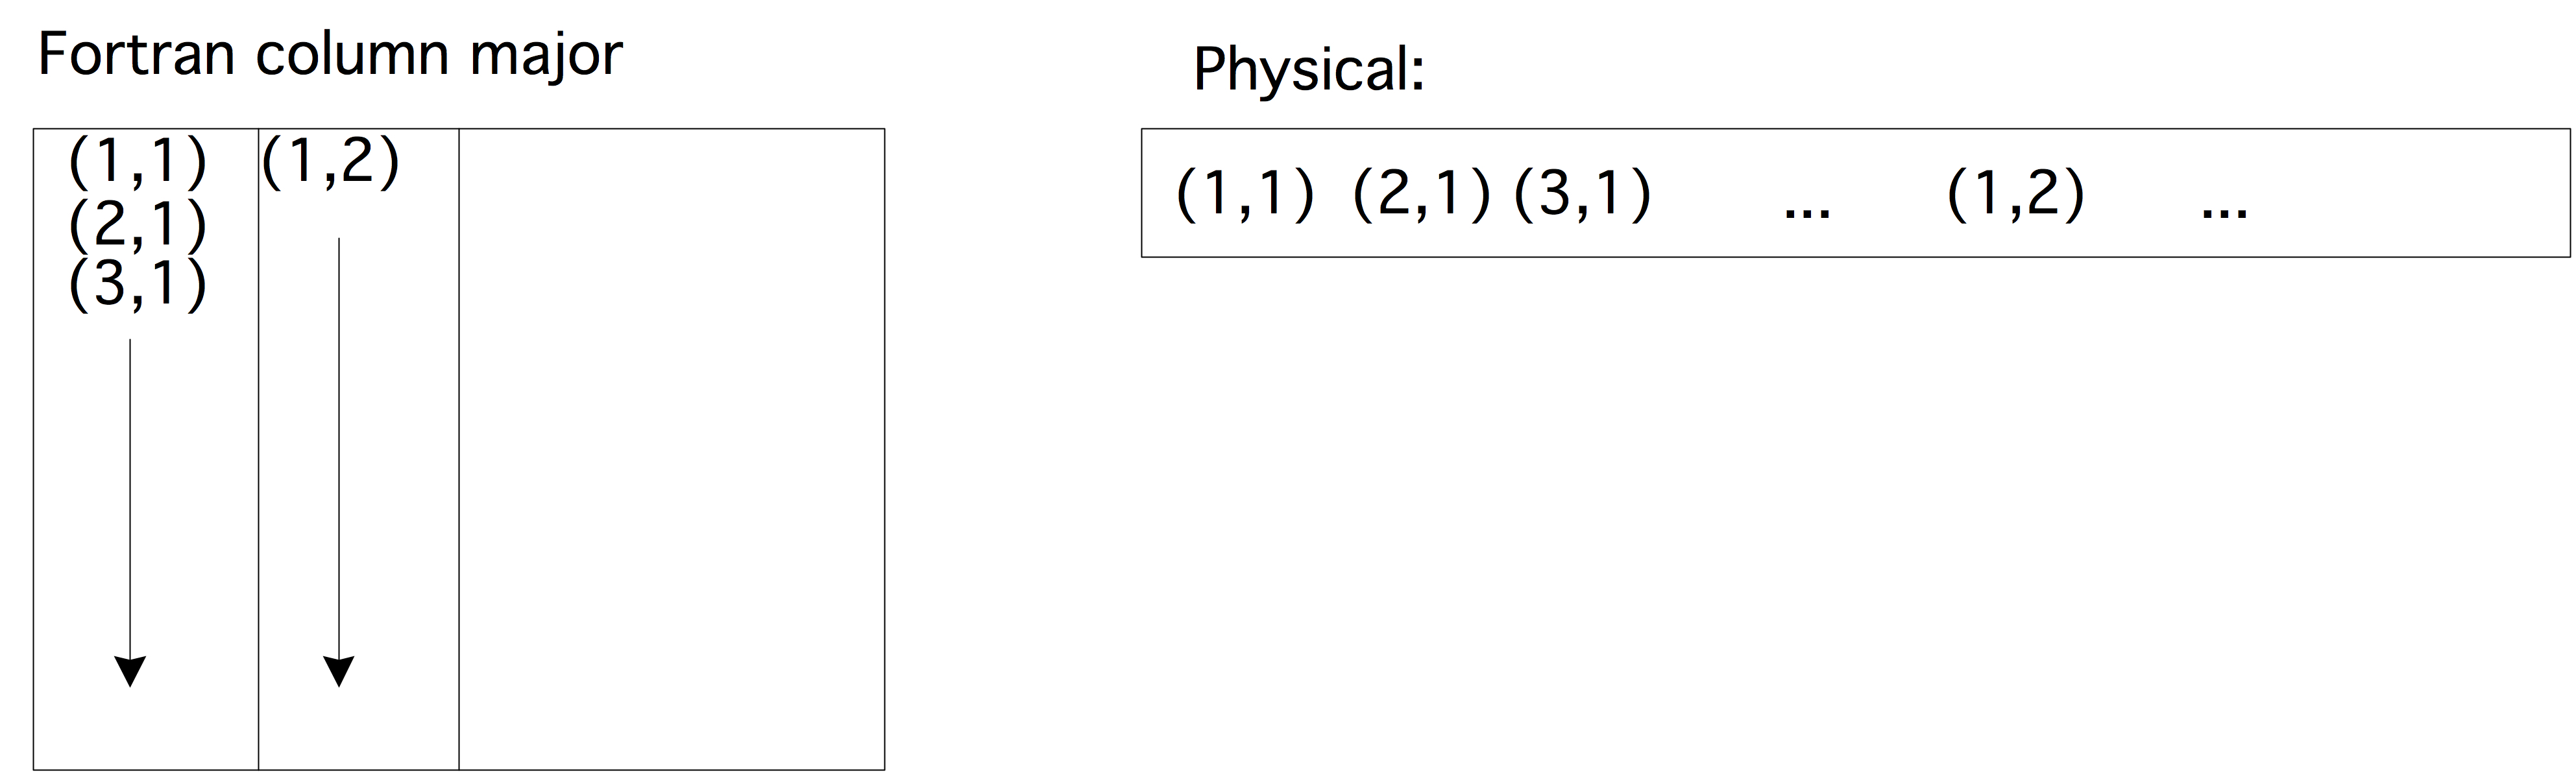
\includegraphics[scale=.1]{arraybycol}

  `First index varies quickest'
\end{slide}

\begin{exercise}
  Can you describe in words how memory elements are access if you
  would write
\begin{lstlisting}
do row=1,size(A,1)
  do col=1,size(A,2)
    .... A(row,col) .....
  end do
end do
\end{lstlisting}
?
\end{exercise}

You can make sections in multi-dimensional arrays: you need to
indicate a range in all dimensions.

\begin{block}{Array sections in multi-D}
  \label{sl:farray-sectiond}
\begin{lstlisting}
real(8),dimension(10) :: a,b
a(1:9) = b(2:10)
\end{lstlisting}
or
\begin{lstlisting}
logical,dimension(25,3) :: a
logical,dimension(25)   :: b
a(:,2) = b
\end{lstlisting}
You can also use strides.
\end{block}

\begin{block}{Array printing}
  \label{sl:farray-print}
  Fill array by rows:
  \[ \begin{matrix}1&2&\ldots&N\\ N+1&\ldots\\ &\ldots\\ &&&MN
  \end{matrix}
  \]
  %
  \snippetwithoutput{printarray}{arrayf}{printarray}
\end{block}

\Level 1 {Querying an array}

We have the following properties of an array:
\begin{itemize}
\item The bounds are the lower and upper bound in each dimension.
  For instance, after
\begin{lstlisting}
integer,dimension(-1:1,-2:2) :: symm
\end{lstlisting}
the array \n{symm} has a lower bound of~\n{-1} in the first dimension
and \n{-2} in the second. The functions \indextermfortdef{Lbound} and
\indextermfortdef{Ubound} give these bounds as array or scalar:
\begin{lstlisting}
array_of_lower = Lbound(symm)
upper_in_dim_2 = Ubound(symm,2)
\end{lstlisting}

\snippetwithoutput{fsection2}{arrayf}{fsection2}

\item The \emph{extent}\index{extent!of array dimension} is the number
  of elements in a certain dimension, and the
  \emph{shape}\index{shape!of array} is the array of extents.

\item The \indextermfortdef{size} is the number of elements, either for
  the whole array, or for a specified dimension.
\begin{lstlisting}
integer :: x(8), y(5,4)
size(x)
size(y,2)
\end{lstlisting}
\end{itemize}

\begin{slide}{Query functions}
  \label{sl:farray-query}
  \begin{itemize}
  \item Bounds: \indextermfort{lbound}, \indextermfort{ubound}
  \item \indextermfort{size}
  \item Can be used per dimension, or overall giving array of bounds/sizes.
  \end{itemize}
  \snippetwithoutput{farrayquery}{arrayf}{query}
\end{slide}

\Level 1 {Reshaping}

\indextermfort{RESHAPE}
\begin{lstlisting}
  array = RESHAPE( list,shape )
\end{lstlisting}
Example:
\verbatimsnippet{shape44}

\indextermfort{SPREAD}
\begin{lstlisting}
  array = SPREAD( old,dim,copies )
\end{lstlisting}

\Level 0 {Arrays to subroutines}

Subprogram needs to know the shape of an array, not the actual bounds:

\begin{block}{Pass array: main program}
  \label{sl:farray-pass1d-main}
  Passing array as one symbol:
  \snippetwithoutput{fpass1dmain}{arrayf}{arraypass1d}
\end{block}

\begin{block}{Pass array: subprogram}
  \label{sl:farray-pass1d-subr}
  Note declaration as \indextermfort{dimension(:)}\\
  actual size is queried
  \verbatimsnippet{fpass1dsubr}
\end{block}

The array inside the subroutine is known as a
\indextermsub{assumed-shape}{array} or
\indextermsub{automatic}{array}.

\Level 0 {Allocatable arrays}
\label{sec:allocatable}

Static arrays are fine at small sizes. However, 
there are two main arguments against using them at large sizes.
\begin{itemize}
\item Since the size is explicitly stated, it makes your program
  inflexible, requiring recompilation to run it with a different
  problem size.
\item Since they are allocated on the so-called \indexterm{stack},
  making them too large can lead to \indextermbus{stack}{overflow}.
\end{itemize}

A better strategy is to indicate the shape of the array, and use
\indextermfort{allocate} to specify
the size later, presumably in terms of run-time program parameters.

\begin{block}{Array allocation}
  \label{sl:farray-alloc}
\begin{lstlisting}
real(8), dimension(:), allocatable :: x,y

n = 100
allocate(x(n), y(n))
\end{lstlisting}
You can \indextermfort{deallocate} the array when you don't need the
space anymore.
\end{block}

If you are in danger of running out of memory, it can be a good idea
to add a \indextermfort{stat=ierror} clause to the \indextermfort{allocate} statement:
\begin{lstlisting}
integer :: ierr
allocate( x(n), stat=ierr )
if ( ierr/=0 ) ! report error
\end{lstlisting}

Has an array been allocated:
\begin{lstlisting}
Allocated( x ) ! returns logical
\end{lstlisting}

Allocatable arrays are automatically deallocated when they go out of
scope. This prevents the \indextermbus{memory}{leak} problems of~C++.

Explicit deallocate:
\begin{lstlisting}
deallocate(x)
\end{lstlisting}

\Level 0 {Array output}

Use implicit do-loops; section~\ref{sec:f-impdo}.

\Level 0 {Operating on an array}

\Level 1 {Arithmetic operations}

Between arrays of the same shape:
\begin{lstlisting}
A = B+C
D = D*E
\end{lstlisting}
(where the multiplication is by element).

\Level 1 {Intrinsic functions}

The following intrinsic functions are avaible for arrays:
\begin{block}{Array intrinsics}
  \label{sl:array-funcf}
  \begin{itemize}
  \item \indextermfort{Abs} creates the matrix of pointwise absolute values.
  \item \indextermfort{MaxVal} finds the maximum value in an array.
  \item \indextermfort{MinVal} finds the minimum value in an array.
  \item \indextermfort{Sum} returns the sum of all elements.
  \item \indextermfort{Product} return the product of all elements.
  \item \indextermfort{MaxLoc} returns the index of the maximum
    element.
  \item \indextermfort{MinLoc} returns the index of the minimum element.
  \item \indextermfort{MatMul} returns the matrix product of two matrices.
  \item \indextermfort{Dot_Product} returns the dot product of two
    arrays.
  \item \indextermfort{Transpose} returns the transpose of a matrix.
  \item \indextermfort{Cshift} rotates elements through an array.
  \end{itemize}
\end{block}

\begin{block}{Multi-dimensional intrinsics}
  \label{sl:array-funcfmd}
  \begin{itemize}
  \item
    Functions such as \indextermfort{Sum} operate on a whole array by
    default.
  \item To
    restrict such a function to one subdimension add a keyword
    parameter \indextermfort{DIM}:
\begin{lstlisting}
s = Sum(A,DIM=1)
\end{lstlisting}
where the keyword is optional.
\item Likewise, the operation can be restricted to a \indextermfort{MASK}:
\begin{lstlisting}
s = Sum(A,MASK=B)
\end{lstlisting}
  \end{itemize}
\end{block}

\begin{exercise}
  \label{ex:fmatnorm}
  The 1-norm of a matrix is defined as the maximum of all sums of absolute
  values in any column:
  \[ \|A\|_1 = \max_j \sum_i |A_{ij}| \]
  while the infinity-norm is defined as the maximum row sum:
  \[ \|A\|_\infty = \max_i \sum_j |A_{ij}| \]
  Compute these norms using array functions as much as possible, that
  is, try to avoid using loops.
  
  For bonus points, write Fortran \lstinline{Function}s that compute
  these norms.
\end{exercise}

\begin{exercise}
  \label{ex:fmatmul}
  Compare implementations of the matrix-matrix product.
  \begin{enumerate}
  \item Write the regular \n{i,j,k} implementation, and store it as
    reference.
  \item Use the \indextermfort{DOT_PRODUCT} function, which eliminates the \n{k}
    index. How does the timing change? Print the maximum absolute
    distance between this and the reference result.
  \item Use the \indextermfort{MATMUL} function. Same questions.
  \item Bonus question: investigate the \n{j,k,i} and \n{i,k,j}
    variants. Write them both with array sections and individual array
    elements. Is there a difference in timing?
  \end{enumerate}
  Does the optimization level make a difference in timing?
\end{exercise}

\Level 1 {Restricting with \tt{where}}

If an array operation should not apply to all elements, you can
specify the ones it applies to with a \indextermfort{where} statement.

\begin{block}{Operate where}
  \label{sl:farray-where}
\begin{lstlisting}
where ( A<0 ) B = 0
\end{lstlisting}

Full form:
\begin{lstlisting}
WHERE ( logical argument )
  sequence of array statements
ELSEWHERE
  sequence of array statements
END WHERE
\end{lstlisting}
\end{block}

\Level 1 {Global condition tests}

Reduction of a test on all array elements:
\indextermfort{all}
\begin{lstlisting}
REAL(8),dimension(N,N) :: A
LOGICAL :: positive,positive_row(N),positive_col(N)
positive = ALL( A>0)
positive_row = ALL( A>0,1 )
positive_col = ALL( A>0,2 )
\end{lstlisting}

\begin{exercise}
  Use array statements (that is, no loops) to fill a two-dimensional
  array~\n{A} with random numbers between zero and~one. Then fill two
  arrays \n{Abig} and \n{Asmall} with the elements of~\n{A} that are
  great than~$0.5$, or less than~$0.5$ respectively:
  \[ A_{\scriptstyle\mathrm{big}}(i,j) =
  \begin{cases}
    A(i,j)&\hbox{if $A(i,j)\geq 0.5$}\\ 0&\hbox{otherwise}
  \end{cases}
  \]
  \[ A_{\scriptstyle\mathrm{small}}(i,j) =
  \begin{cases}
    0&\hbox{if $A(i,j)\geq 0.5$}\\ A(i,j)&\hbox{otherwise}
  \end{cases}
  \]
  Using more array statements, add \n{Abig} and \n{Asmall}, and test
  whether the sum is close enough to~\n{A}.
\end{exercise}

Similar to \indextermfort{all}, there is a function~\indextermfort{any} that tests
if any array element satisfies the test.
\begin{lstlisting}
if ( Any( Abs(A-B)>
\end{lstlisting}

\Level 0 {Array operations}

\Level 1 {Loops without looping}

In addition to ordinary do-loops, Fortran has mechanisms that save you
typing, or can be more efficient in some circumstances.

\Level 2 {Slicing}

If your loop assigns to an array from another array,
  you can use section notation:
\begin{lstlisting}
a(:) = b(:)
c(1:n) = d(2:n+1)
\end{lstlisting}

\Level 2 {`forall' keyword}

The \indextermfort{forall} keyword also indicates an array assignment:
\begin{lstlisting}
forall (i=1:n)
  a(i) = b(i)
  c(i) = d(i+1)
end forall
\end{lstlisting}
You can tell that this is for arrays only, because the loop index has
to be part of the left-hand side of every assignment.

This mechanism is prone to misunderstanding and therefore now
deprecated.
It is not a parallel loop! For that, the following mechanism is preferred.

\Level 2 {Do concurrent}

\begin{block}{Do concurrent}
  \label{sl:farray-concurrent}

  The \indexterm{do concurrent} is a true do-loop. With the
  \indextermfort{concurrent} keyword the user specifies that the
  iterations of a loop are independent, and can therefore possibly be
  done in parallel:
\begin{lstlisting}
do concurrent (i=1:n)
  a(i) = b(i)
  c(i) = d(i+1)
end do
\end{lstlisting}
(Do not use \indextermfort{for all})
\end{block}

\Level 1 {Loops without dependencies}

Here are some illustrations of simple array copying with the above
mechanisms.

\verbatimsnippet{blockrecur}
\begin{lstlisting}
Original     1   2   3   4   5   6   7   8   9  10
Recursive    0   2   4   6   8  10  12  14  16  18
\end{lstlisting}

\verbatimsnippet{blockslice}
\begin{lstlisting}
Original     1   2   3   4   5   6   7   8   9  10
Section      0   2   4   6   8  10  12  14  16  18
\end{lstlisting}

\verbatimsnippet{blockforall}
\begin{lstlisting}
Original     1   2   3   4   5   6   7   8   9  10
Forall       0   2   4   6   8  10  12  14  16  18
\end{lstlisting}

\verbatimsnippet{blockconc}
\begin{lstlisting}
Original     1   2   3   4   5   6   7   8   9  10
Concurrent   0   2   4   6   8  10  12  14  16  18
\end{lstlisting}

\begin{exercise}
  Create arrays \n{A,C} of length~\n{2N}, and \n{B}~of length~\n{N}.
  Now implement
  \[ B_i = (A_{2i}+A_{2i+1})/2,\quad i=1,\ldots N \]
  and
  \[ C_i = A_{i/2},\quad i=1,\ldots 2N \]
  using all four mechanisms. Make sure you get the same result every time.
\end{exercise}

\Level 1 {Loops with dependencies}

For parallel execution of a loop, all iterations have to be independent.
This is not the case if the loop has a \indexterm{recurrence}, and in
this case, the `do concurrent' mechanism is not appropriate.
%
Here are the above four constructs, but applied to a loop with a dependence.
%
\verbatimsnippet{slicerecur}
%
\begin{lstlisting}
Original   1   2   3   4   5   6   7   8   9  10
Recursiv   1   2   4   8  16  32  64 128 256 512
\end{lstlisting}

The slicing version of this:
%
\verbatimsnippet{sliceslice}
%
\begin{lstlisting}
Original   1   2   3   4   5   6   7   8   9  10
Section    1   2   4   6   8  10  12  14  16  18
\end{lstlisting}
%
acts as if the right-hand side is saved in a temporary array, and
subsequently assigned to the left-hand side.

Using `forall' is equivalent to slicing:
%
\verbatimsnippet{sliceforall}
%
\begin{lstlisting}
Original     1   2   3   4   5   6   7   8   9  10
Forall       1   2   4   6   8  10  12  14  16  18
\end{lstlisting}

On the other hand, `do concurrent' does not use temporaries, so it is
more like the sequential version:
%
\verbatimsnippet{sliceconc}
%
\begin{lstlisting}
Original     1   2   3   4   5   6   7   8   9  10
Concurrent   1   2   4   8  16  32  64 128 256 512
\end{lstlisting}
Note that the result does not have to be equal to the sequential
execution: the compiler is free to rearrange the iterations any way it
sees fit.

\Level 0 {Review questions}

\begin{exercise}
  \label{ex:farray-assign-section}
  Let the following declarations be given, and assume that all arrays
  are properly initialized:
\begin{lstlisting}
real                   :: x
real, dimension(10)    :: a, b
real, dimension(10,10) :: c, d
\end{lstlisting}

Comment on the following lines: are they legal, if so what do they do?
\begin{enumerate}
\item \n{a = b}
\item \n{a = x}
\item \n{a(1:10) = c(1:10)}
\end{enumerate}

How would you:
\begin{enumerate}
\item Set the second row of \n{c} to~\n{b}?
\item Set the second row of \n{c} to the elements of~\n{b}, last-to-first?
\end{enumerate}
\end{exercise}
